\documentclass[12pt,twoside,titlepage]{ingenius}
\usepackage[figuresright]{rotating}
\usepackage{pgfplots} 
\pgfplotsset{compat=1.7}
\usepackage{adjustbox}
\usepackage{units}
\usepackage{dblfloatfix}
\usepackage{amssymb}
\usepackage{caption}
\usepackage{subcaption}
\usepackage{bm}
\usepackage{textcomp}
\usepackage{pifont}
\usepackage{cite}
\usepackage{xcolor,colortbl}
\usepackage{amsmath}
\usepackage{upgreek}
\usepackage{graphicx}
\usepackage{tikz}%flujogramas
\usepackage{pifont}
\usetikzlibrary{shapes,arrows}
\usepackage{textcomp}
\usepackage{multirow}
\usepackage{float}
\usepackage{soul}
\usepackage{rotating}
\usepackage{hyperref}
\usepackage{booktabs}
\usepackage{algorithmic}
\usepackage[ruled,vlined,algo2e]{algorithm2e}
\usepackage{algorithm}
%\usepackage{fancyhdr}
%\pagestyle{fancy}
\makeatletter
\renewcommand*{\ALG@name}{Algoritmo}
\makeatother
\graphicspath{{figures/}}
%===========================================
%========
\usepackage{tikz,xcolor,hyperref}
% Make Orcid icon
\definecolor{lime}{HTML}{A6CE39}
\DeclareRobustCommand{\orcidicon}{%
	
\begin{tikzpicture}
	\draw[lime, fill=lime] (0,0) 
	circle [radius=0.16] 
	node[white] {{\fontfamily{qag}\selectfont \tiny ID}};
	\draw[white, fill=white] (-0.0625,0.095) 
	circle [radius=0.007];
	\end{tikzpicture}
	\hspace{-2mm}
}
\foreach \x in {A, ..., Z}{%
	\expandafter\xdef\csname orcid\x\endcsname{\noexpand\href{https://orcid.org/0009-0006-0590-6700}{\noexpand\orcidicon}}
}
%========================================================
\titulo{Inteligencia artificial y accesibilidad educativa en lenguas de bajos recursos: una revisión sistemática de usos, desafíos y oportunidades}
\tituloa{A Systematic Review of Artificial Intelligence for Improving Educational Accessibility in Low-Resource Languages: Uses, Challenges, and Opportunities}
%========================================================
\newcommand{\orcidauthorA}{0000-0002-7645-8793}
\newcommand{\orcidauthorB}{0000-0002-0837-0642}
\newcommand{\orcidauthorC}{0000-0002-4704-1067}
\autores{Lorena Kim Negrillo $^{1}$,\orcidA{}}
\adscripcionautor{%
$^{1}$ Lorena Kim Negrillo, Faculdad de Ingeniería de Software, Universidad Tecnológica del Perú, Lima, Perú, e-mail: U22229186@utp.edu.pe\\
}

%%Datos para referencias
\newcommand{\apellido}{Kim Negrillo.}% Apellido o apellidos para referencia 
\newcommand{\titu}{Revisión sistemática sobre inteligencia artificial para mejorar la accesibilidad educativa en lenguas de bajos recursos: usos, desafíos y oportunidades}%titulo a la ref\erencia
\newcommand{\tipo}{Art\'iculo Cient\'if{}ico / Scientif{}ic Paper} 
%tipo de documento Punto de vista/Point of view,  Art\'iculo Cient\'if{}ico / Scientif{}ic Paper, Rese\~na bibliogr\'afica/Review
%========================================================
%%Datos para propiedades del pdf no requiere ser llenado
\newcommand{\autor}{}%autor para propiedades del pdf
\newcommand{\pc}{}%palabras clave para propiedades del pdf
\newcommand{\kw}{}%keywords para propiedades del pdf
\usepackage{xcolor}
\usepackage{color}
\input{configuracion_paquetes}
%\input{config_c}
\usepackage{listings}%% lista de códigos
	\lstset{ 
		linewidth=0.5\textwidth,
		frame=tb,	
		%framerule=0.5pt,
		aboveskip=0.5cm,%Distancia Texto al codigo
		%framextopmargin=3pt,%Distancia Primera Linea-Borde Superior
		framexbottommargin=3pt,%Distancia Ultima Linea-Borde Inferior
		%framexleftmargin=0.4cm,%Distancia Borde Izquierdo Codigo-Borde Izquierdo Pagina
		framesep=0pt,
		rulesep=.8pt,%Espesor linea junto a los numeros
		backgroundcolor=\color{gray!10},
                     numbersep=5pt,
                     xleftmargin=3pt,
                     xrightmargin=8.5pt,
                     framextopmargin=10pt,
		rulesepcolor=\color{black},
		stringstyle=\ttfamily,
		floatplacement=htb,
		boxpos={c},
		breaklines=true,
		breakatwhitespace=true,
		showstringspaces = false,
		basicstyle=\small\ttfamily,
		commentstyle=\color{gray!45},
		keywordstyle=\bfseries,
		%linewidth=0.8\textwidth,
		title=\lstname,
		%numbers=right,%Posicion de los Numeros left=izquierda; right=derecha
		%numbersep=15pt, %separacion de numero 1,2,3,4 hacia el frame
		numberstyle=\tiny,
		numberfirstline = false,
		breaklines=true,
		}
	\lstnewenvironment{listing}[1][]
		{\lstset{#1}\pagebreak[0]}{\pagebreak[0]}
		\lstdefinestyle{consola}
		{basicstyle=\scriptsize\bf\ttfamily,
		 backgroundcolor=\color{gray75},
		}
	\lstdefinestyle{C}
		{language=C,
}

\newenvironment{tabla}
  {\par\bigskip\noindent\minipage{\linewidth}}
  {\endminipage\par\bigskip}

\newenvironment{figura}
  {\par\bigskip\noindent\minipage{\linewidth}}
  {\endminipage\par\bigskip}

\newenvironment{pseudo}
  {\par\noindent\minipage{\linewidth}}
  {\endminipage\par\bigskip}
%========================================================
\begin{document}
\renewcommand{\lstlistingname}{Algorithm}
\setcounter{page}{1}
\renewcommand{\refname}{Referencias}
\renewcommand{\figurename}{Figura}
\renewcommand{\tablename}{Tabla}
\frenchspacing

% \begin{tikzpicture}[overlay]
%  \node at (138mm,2mm){\textsf{\scriptsize pISSN: 1390-650X / eISSN: 1390-860X}};
% \end{tikzpicture}

\input{silabeo}
\membrete
\input{configuracion_portada}

%\begin{textblock}{12.4}(0,10)
\begin{textblock}{12.4}(0,10)%Modificar Editor Ingenius cuando se inserte Creative Commons
\adscripcion
\end{textblock}
%========================================================
\begin{table}[htb]
\begin{tabular}{p{8cm}p{8cm}}
{\Large \bfseries Resumen} &{\Large \bfseries Abstract} \\ \\

Bajo el marco de trabajo PRISMA, se realizó una revisión sistemática de la literatura en la base de datos Scopus, donde se analizaron 27 artículos publicados entre los años 2022 y 2026. Los resultados revelaron que si bien modelos multilingües no se desempeñan correctamente en lenguas de bajos recursos, por ejemplo, el modelo \textit{Cross-Lingual Language Modeling-Roberta}(XLM-R) en un escenario \textit{zero-shot} sobre 10 lenguas indígenas obtuvo una presición promedio de 38.48\%, existen enfoques que permiten obtener resultados más favorables, como el uso de meta-aprendizaje (MAML), implementación de arquitecturas hibridas, inyección de conocimiento lingüistico y un enfoque participativo con la población de estudio. Aún existen limitaciones que son necesarias de abarcar en futuras investigaciones, como la escacez de datos y falta de recursos computacionales, la necesidad de un enfoque participativo y métricas especializadas para lenguas de bajos recursos lingüisticos, por tal motivo se sugiere que los investigadores adopten enfoques participativos y prioricen las necesidades con los hablantes de las lenguas estudiadas.

&Under the PRISMA methodology, a systematic literature review was conducted using the Scopus database, in which 27 articles published between 2022 and 2026 were analyzed. The results revealed that, although multilingual models do not perform adequately in low-resource languages—for example, the \textit{Cross-Lingual Language Modeling-Roberta} (XLM-R) model achieved an average accuracy of 38.48\% in a \textit{zero-shot} scenario across 10 Indigenous languages—there are approaches that make it possible to obtain more favorable results, such as the use of meta-learning (MAML), the implementation of hybrid architectures, the injection of linguistic knowledge, and a participatory approach involving the study population. There are still limitations that need to be addressed in future research, such as data scarcity and the lack of computational resources, the need for a participatory approach, and specialized metrics for low-resource languages. Therefore, it is suggested that researchers adopt participatory approaches and prioritize needs together with the speakers of the languages being studied.
% Debe contener un máximo de 230 palabras, no debe incluir ecuaciones o referencias. El contenido del resumen debe estar completamente justificado.
……………..
\\[-0.3cm]
\palabrasclave{Aprendizaje, aprendizaje personalizado, enseñanza, equidad educativa, Inteligencia Artificial, lenguas con pocos recursos, pedagogía, procesamiento del lenguaje natural.}&\keywords{Artificial Intelligence, educational equity, learning, low-resource languages, natural language processing, pedagogy, personalized learning, teaching.}  \\
\end{tabular}
\end{table}

\newpage


\begin{multicols}{2}
\raggedcolumns
%========================================================
\section{Introducción}
\vspace{-0.15cm}

% contexto, problema, justificación, objetivos

La Organización de las Naciones Unidas para la Educación, la Ciencia y la Cultura (UNESCO) señala que el 40\% de la población mundial no tiene acceso a
educación en una lengua que hable y comprenda con fluidez. Si bien este problema afecta a la población en general, su impacto en las personas cuyas lenguas
maternas corresponden a lenguas de bajos recursos es mucho más drástico  \cite{UNESCO}. Una de las principales dificultades en el ámbito educativo es la persistencia de barreras lingüísticas que limitan el acceso equitativo al aprendizaje a estudiantes cuya lengua materna corresponde a una lengua de bajos recursos lingüísticos, como el quechua o el aimara, debido a la limitada información existente, complejidad morfológica y superposiciones semánticas \cite{Demilie2026,Tafa2025}. 


En torno a esta problemática, la inteligencia artificial (IA) ha comenzado a posicionarse como una alternativa con alto potencial para enfrentar estas limitaciones y se ha venido consolidando como una vía prometedora para mejorar la accesibilidad y personalización del aprendizaje. 
Asimismo, revisiones recientes en el campo de la educación lingüística muestran que las herramientas basadas en IA, incluidos los sistemas
conversacionales y los grandes modelos de lenguaje, han ampliado las posibilidades de apoyo pedagógico en contextos multilingües, aunque todavía existen desafíos significativos en términos de equidad, calidad y estabilidad de los resultados educativos \cite{BeldaMedina2022,Nwafor2026,Nouzri2025,Tebourbi2025}.


En particular, los grandes modelos de lenguaje, \textit{LLMs}, por sus siglas en inglés, tales como ChatGPT o Gemini demuestran un gran desempeño en trabajos que requieren procesamiento del lenguaje natural, sin embargo, su rendimiento en tareas que requieren de un razonamiento más explícito, aún constituye un ámbito inexplorado y con varias inconsistencias. En \cite{Onan2026} se realizó un estudio que comparó seis \textit{LLMs} usados para preguntas de un examen en turco e indonesio, los resultados mostraron que mientras GPT-4 produce las explicaciones de mayor calidad y alineación pedagógica de manera más consistente, Gemini y Qwen 3 logran un desempeño competitivo, pero menos estable en categorías cognitivas, y por su parte DeepSeek-V2 tiene un desempeño sólido en tareas de razonamiento, pero muestra una menor estabilidad temporal, en contraste, Copilot y Phi-2 muestran un menor rendimiento en tareas de pensamiento complejo. Tales hallazgos tienen implicancias directas para la equidad educativa, el rendimiento estudiantil y la educación de calidad en contextos de bajos recursos, especialmente en entornos donde las herramientas basadas en IA son el principal recurso de aprendizaje. 


De manera complementaria, trabajos recientes muestran que estas tecnologías también se están explorando en contextos de aprendizaje de lenguas mediante sistemas multiagente, asistentes conversacionales y flujos de aprendizaje personalizados \cite{Nouzri2025,Tebourbi2025}. Estas evidencias son relevantes para las lenguas de bajos recursos, sugieren que la utilidad educativa de la IA depende tanto de la potencia del modelo como de su adaptación lingüística y pedagógica al contexto de uso.


En este contexto, resulta relevante examinar no solo la capacidad lingüística de los modelos, sino también su utilidad pedagógica y su estabilidad en contextos multilingües. En ese sentido, \cite{Onan2026} señala que una limitación predominante en las investigaciones actuales es el enfoque casi exclusivo en lenguas de alto recurso, tales como el inglés, lo que deja un vacío significativo en la comprensión de cómo estas tecnologías pueden aplicarse en lenguas de bajos recursos. Esto, a su vez, limita el desarrollo de soluciones efectivas y contextualizadas para estos grupos lingüísticos.


De igual manera, en una revisión sistemática orientada a examinar el panorama actual de la investigación sobre IA generativa en la educación del idioma árabe \cite{Moustafa2026}, se evidenció la escasez de recursos académicos luego de recuperar inicialmente 87 registros en bases de datos globales como Scopus y Web of Science, de los cuales únicamente 4 estudios, que representan apenas el 4.6\%, cumplieron con los criterios de inclusión pedagógica y empírica. Aunque se centra en un contexto lingüístico particular, este hallazgo permite inferir que la evidencia disponible sobre el uso de la IA en entornos educativos multilingües todavía es escasa.


A pesar de que la inteligencia artificial en la educación constituye un campo en expansión, la literatura científica disponible todavía se encuentra dispersa. Mientras algunas investigaciones se centran en el desempeño técnico de modelos de traducción, otras analizan experiencias de uso educativo de la IA sin centrarse específicamente en lenguas de bajos recursos ni en la reducción de barreras lingüísticas. Debido a esto, aún no se observan con suficiente claridad los enfoques que han sido más utilizados, qué resultados educativos se han reportado y cuáles son los principales retos metodológicos, éticos y tecnológicos en este campo. 


Dada la dispersión temática y metodológica de la evidencia disponible, resulta necesaria una revisión sistemática de la literatura que permita esclarecer el estado actual del conocimiento, identificar tendencias, oportunidades y vacíos de investigación, así como reconocer las estrategias y metodologías más eficaces, particularmente en contextos educativos donde las tecnologías emergentes pueden contribuir a promover la equidad y la innovación, como también se señala en \cite{Yoshida2025}.


En respuesta a esta necesidad, se plantea una revisión sistemática de la literatura científica sobre el uso de la inteligencia artificial para mejorar la accesibilidad educativa en lenguas de bajos recursos, con especial atención a la reducción de barreras lingüísticas. Esta revisión tiene como propósito sintetizar los enfoques metodológicos empleados, los resultados educativos reportados y los principales desafíos y oportunidades identificados en la literatura, a fin de ofrecer una visión integral del estado actual del campo y orientar futuras investigaciones.

\section{Metodología}

Para el desarrollo del estudio, se adoptó el enfoque de Revisión Sistemática de la Literatura (RSL) con el propósito de recopilar, evaluar y sintetizar el material científico disponible acerca de las aplicaciones basadas en inteligencia artificial para la mejora de accesibilidad educativa en lenguas de bajos recursos. A su vez, se decidió usar la metodología PRISMA, una guía publicada en el año 2009 que marca un estándar de calidad para la elaboración de revisiones sistemáticas, garantizando transparencia, rigor y calidad de presentación. 
Asimismo, se empleó el marco de trabajo PICO (Población, Intervención, Comparación y Resultado) para delimitar con presición el alcance del estudio. Los componentes que integran este marco se definieron de la siguiente manera:

\begin{itemize}
   \item P: Estudiantes cuya lengua materna es una lengua de bajos recursos.
   \item I: Uso de herramientas basadas en Inteligencia Artificial (IA), grandes modelos de lenguaje (LLMs).
   \item C: Desempeño en lenguas de altos recursos.
   \item O: Mejora en la accesibilidad, personalización del aprendizaje, equidad educativa e innovación pedagógica.
\end{itemize}

A partir de esto, se formularon preguntas específicas que vinculen las lenguas de bajos recursos con Inteligencia Artificial (IA). Las preguntas formuladas se detallan en la tabla 1:


\begin{table}[H]
\centering
\captionof{table}{Estructura PICO}
\small
    \begin{tabular}{cp{4.6cm}}
    \toprule
    \multicolumn{1}{c}{\textbf{Esquema PICO}} & \multicolumn{1}{c}{\textbf{Preguntas}} \\
    \midrule
    P & ¿De qué manera las tecnologías de Procesamiento de Lenguaje Natural (NLP) benefician la integración de la lengua materna en entornos educativos? \\ \addlinespace
    I & ¿De qué manera las herramientas basadas en IA y LLMs mejoran la accesibilidad educativa? \\ \addlinespace
    C & ¿Qué vacíos existen entre el desempeño de la IA en lenguas de alto recurso frente a las de bajos recursos? 
 \\ \addlinespace
    O & ¿Qué estrategias y metodologías son las más eficaces para mejorar la accesibilidad educativa?
 \\
    \bottomrule
    \end{tabular}%
  \label{tabla1}%
\end{table}

De igual forma, la estrategia de búsqueda elaborada se basó en artículos procedentes únicamente de la base de datos Scopus, una de las bases de datos más prestigiosas a nivel mundial. Para la selección de artículos, se establecieron los siguientes criterios:

\begin{itemize}
   \setlength{\itemsep}{0pt}
   \setlength{\parskip}{0pt}
   \item Criterio 1 (C1): Estudios realizados en estudiantes cuya lengua nativa es de de bajos recursos.
   \item Criterio 2 (C2): Estudios que empleen IA, LLMs o Natural Language Processing (NLP).
   \item Criterio 3 (C3): Desempeño de herramientas basadas en IA en lenguas de altos recursos.
   \item Criterio 4 (C4): Estudios cuyo propósito sea mejorar la accesibilidad, mejorar el aprendizaje o promover la equidad educativa y pedagógica.
   \item Criterio 5 (C5): Estudios de áreas relacionadas a Ciencias de la Computación, Artes y Humanidades, Ciencias Sociales, Ingeniería y Matemáticas.
\end{itemize}

Asimismo, la tabla 2 detalla la metodología empleada para la búsqueda: se presenta la pregunta de investigación formulada en base a las preguntas del esquema PICO, palabras clave identificadas, ecuación general de búsqueda y los criterios de selección empleados, más adelante siendo usados en la exclusión de artículos.


\begin{table}[H]
\centering
\captionof{table}{Metodología usada para la búsqueda}
\small
\begin{tabular}{|p{2cm}|p{5.3cm}|}
\hline
\centering{Parámetros de búsqueda} 
& \centering\arraybackslash{Parámetros de búsqueda de la información} \\
\hline

{Pregunta de investigación} 
& ¿De qué manera la integración de la Inteligencia Artificial impacta en la accesibilidad educativa y la calidad de la información recuperada por estudiantes de lenguas de bajos recursos, en comparación con lenguas de altos recursos? \\
\hline

{Palabras clave} 
& Low-resource languages, minority languages, linguistic barriers, Artificial intelligence, large language models, natural language processing, high-resource languages, thematic dispersion,  Educational accessibility, educational equity, personalized learning, pedagogy. \\
\hline

{Base de datos} 
& Scopus. \\
\hline

{Intervalo de fechas} 
& 2022--2026. \\
\hline

{Ecuación general de búsqueda} 
& 
("Artificial Intelligence" OR AI OR "Large Language Models" OR LLM* OR "Natural Language Processing" OR "NLP" OR "Machine Learning" OR "Generative AI" OR "Machine Translation" OR "Language Technolog*")
AND
("low-resource language*" OR "under-resourced language*" "minority language*" OR "indigenous language*" OR "linguistic barrier*" OR "endangered language*" OR "language barrier*" OR Quechua OR Aymara)
AND
("educational accessibility" OR "educational equity" OR "personalized learning" OR education* Or teach* Or learn* OR pedagog*) \\
\hline

{Idioma}
&
Inglés. \\
\hline

{Tipo de documento}
&
Artículo, conference paper, revisiones. \\
\hline

{Accesibilidad}
&
Open access. \\
\hline

{Criterios de selección}
&
Estudios que aborden el uso de inteligencia artificial en el procesamiento, enseñanza o accesibilidad de lenguas de bajos recursos o lenguas de altos recursos.  \\
\hline

\end{tabular}
\label{tabla:parametros_busqueda}
\end{table}

La búsqueda en Scopus identificó 118 artículos, de los cuales 87 fueron excluidos debido a su antigüedad, falta de acceso abierto o ser capítulos de libros. De los 31 restantes, 4 no cumplieron con el criterio 5 de inclusión. Finalmente, pudo recuperarse un total de 27 artículos. La figura 1 muestra el diagrama PRISMA que detalla el proceso completo (identificación, evaluación y selección).

\begin{figure}[H]
\begin{center}
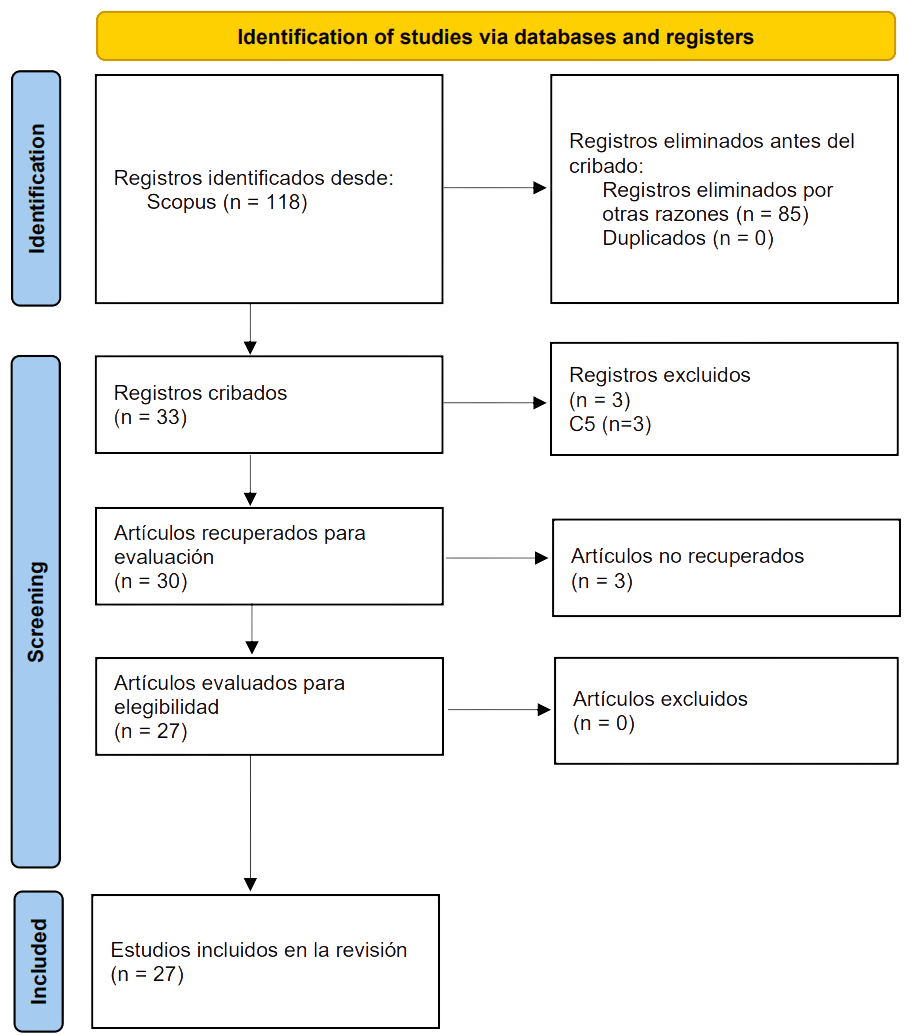
\includegraphics[width=7.8cm]{figures/fig1.png}
\end{center}
\caption{Diagrama de Prisma}
\label{figura1}
\end{figure}


% Las secciones de Introducción, Materiales y Métodos, Resultados y Discusión y Conclusiones del artículo pueden estructurarse divididas en diferente forma. En cada epígrafe del artículo se deben enumerar como máximo hasta tres niveles: 1. / 1.1. / 1.1.1. En esta plantilla en la sección materiales y métodos se explica cada una de las partes del manuscrito y como elaborarlo.

% \subsection{Título principal}

% El título principal (en la primera página) debe estar centrado, se debe respetar el codigo establecido para el efecto, respetando además el orden de mayusculas y minusculas, ya que el mismo se mostrará después de la compilación con la tipografía de fuente \textsc{Versalitas}.

% \subsection{Nombre del Autor(s) y afiliaciones}

% Los nombres del autor(es) deben estar centrados abajo del título y deben ser ingresados en el código indicado, tal como se indica en la parte superior de este documento.
%       Se escribirá primero el nombre y luego el apellido. En el caso de que el artículo tenga más de un autor, los nombres estarán separados por comas de manera que todos los nombres se los autores estén en una sola línea. Los detalles de los autores no deben mostrar ningún título profesional como PhD, MSc, Dr.

% \subsection{Títulos de primer, segundo y tercer nivel}

% El primer nivel corresponde al título principal de cada epígrafe, use el comando "\emph{section}", se debe usar un punto después del número del título.

% El segundo nivel corresponde a los subtitulos use el comando "\emph{subsection}"; mientras que para los subtitulos de tercer nivel use el comando "\emph{subsubsection}" 

% La configuración de esta plantilla permitirá que en cada nivel se muestre el tamaño de texto que identifique a cada uno.

% \subsection{Texto principal}

% El texto principal del artículo deberá ser colocado respetando las reglas gramaticales la condiguración de la plantilla mostrará los espaciados, tipo de fuente, sangrías, etc.

% \subsection{Figuras, tablas, ecuaciones, unidades y abreviaturas.}

% Figuras: Todas las figuras deben estar cargadas en la carpeta del código fuente denominada "\emph{figures}" con un nombre caracteristico que identifique a cada figura que conste en el artículo, utilice el código a continuación indicado para llamar a cada figura según corresponda en el texto del artículo, de la misma manera en el campo "\emph{caption}" colocar el nombre de la figura. Las figuras pueden estar en formato .jpg .png o .pdf con una resolución mínima de 300 dpi (ver Figura \ref{figura1}). También se pueden insertar código para figuras que usen el paquete TiKz o Pgfplots como muestra la Figura \ref{figura2}. Todas las figuras deben estar citadas en el texto. Si la figura posee dos partes incluya los indicativos “(a)” y “(b)” 

% \begin{figure}[H]
% \begin{center}
% 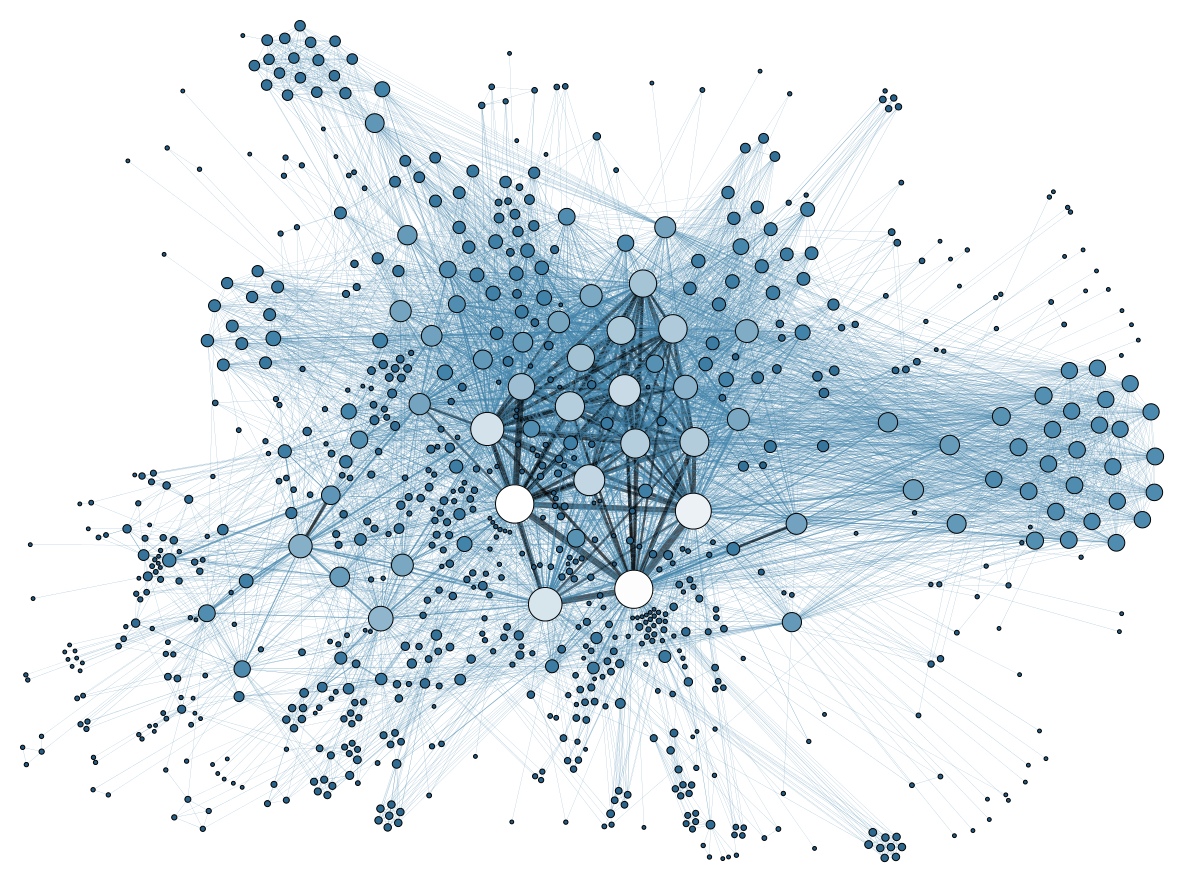
\includegraphics[width=7.8cm]{figures/fig2.png}
% \end{center}
% \caption{Nombre de la Figura.\cite{Mahmood2015}}
% \label{figura1}
% \end{figure}

% \begin{figure}[H]
% \centering
% %\label{fig2}
% \resizebox{6cm}{!} {
% \begin{tikzpicture}%
%    \begin{axis}[
%       ylabel style={overlay},
%       yticklabel style={overlay},
%       xlabel={$x$},
%       ylabel={$y$},
%       legend style={at={(0.5,0.97)},
%          anchor=north,legend columns=-1},
%       domain=-2:2
%    ]
%    \addplot {x^2};
%    \addplot {x^3};
%    \addplot {x^4};
%    \legend{$x^2$,$x^3$,$x^4$}
%    \end{axis}
% \end{tikzpicture}
% }
% \caption{El título}
% \label{figura2}
% \end{figure}

% Tablas: Coloque las tablas al inicio o al final de las columnas. A diferencia de las figuras el título de las tablas se coloca en la parte superior de la misma. 
% En la Tabla \ref{tabla1} de esta guía se muestra un ejemplo del formato para la presentación del artículo.
% Debe verificar que igual que las figuras, las tablas que se encuentren en el artículo se citen en el texto principal. 

% \begin{table}[H]
% \centering
% \captionof{table}{Tamaños de Fuente que se utilizan en la plantilla de articulos de la revista INGENIUS}
%   \scalebox{0.74}{
%     \begin{tabular}{cl}
%     \toprule
%     \multicolumn{1}{c}{Tamaño de letra} & \multicolumn{1}{c}{Uso} \\
%     \midrule
%     \small{10}    & \small{Datos del autor, título, texto de tablas y figuras.} \\
%     {\textbf{12}} & \textbf{Resumen, palabras clave} \\
%     12    & Nombre del autor(es), texto del artículo  \\
%     \Large{13}    & \Large{Títulos de segundo y tercer orden} \\
%     \LARGE{\textbf{15}} & \LARGE{\textbf{Títulos de primer nivel}} \\
%     \huge{\textbf{18}} & \huge{\textbf{TITULO}} \\
%     \bottomrule
%     \end{tabular}%
% }
%   \label{tabla1}%
% \end{table}

% Ecuaciones: Utilice editor de ecuaciones desde OverLeaf.  Trate de que las ecuaciones sean compactas empleando en el signo (/), la función exponencial como exp, o subíndices y superíndices. Las ecuaciones requeridas dentro del modelo matemáticas serán enumeradas según se detalla a continuación en la Ec \ref{eq1}.

% \begin{equation} 
% \label{eq1}
% \begin{array}{ll}
% \alpha = \frac{l + s}{s} * \lambda & [veh]
% \end{array}
% \end{equation}

% Unidades: Las unidades recomendadas son las del sistema métrico, en particular, se sugiere el uso del Sistema Internacional de Unidades (Unidades SI). Las unidades del sistema inglés pueden emplearse como unidades secundarias (en paréntesis). 

% Abreviaturas: Se deben definir las abreviaturas y acrónimos que no sean comunes la primera vez que aparecen en el texto, aún si ya se han definido en el resumen. No utilice abreviaturas en el título a menos que sea inevitable.

% \subsection{Referencias}

% Se debe verificar con cuidado que todas las citas colocadas en el texto, aparezcan en la lista de referencias bibliográficas. En la lista solo deben aparecer las referencias que fueron utilizadas en el texto principal del trabajo, en las tablas o en las figuras, esto implica que no deben aparecer otras referencias aunque el autor las haya consultado durante la preparación del artículo.

%         Las referencias incluidas en el texto se presentan al final ordenadas numéricamente en paréntesis cuadrados \cite{Valenzuela2019} según el orden de aparición en el texto. Un punto debe seguir al paréntesis \cite{Panwar2019}. Referencias múltiples pueden citarse con paréntesis separados por un guión \cite{Ramirez2015,Pagani2014,Peralta2017}. Cuando se cite un libro indicar las páginas con la información relevante. El título como tal de las “Referencias” al final del artículo no va numerado.
        
% Puede consultar la guía del IEEE para la cita de referencias disponible en el link: \url{https://bit.ly/2PjrnJj}

% Las referencias deben ser guardadas en el archivo \textbf{referencias.bib} en formato bibtex, indicando la \textbf{bibkey} secuencialmente según su aparición. Se recomienda utilizar un gestor bibliográfico para que pueda corregir previamente los metadatos como: autor, título, publisher, volume, issue, año, páginas, en caso de ser incorrectos \textbf{Mendeley}

\section{Resultados}
Los resultados han sido divididos en dos partes: bibliométricos e ingeniería. 

\subsection{Resultados bibliometricos}
Luego del proceso de identificación de documentos científicos especificado en la figura 1, los artículos fueron ordenados según su año de publicación. En la figura 2, se puede identificar cómo en los últimos años el 2025 tuvo la mayor cantidad de producción científica con 10 artículos publicados, lo cual a su vez representa el 37\% con respecto al total.

\begin{figure}[H]
\begin{center}
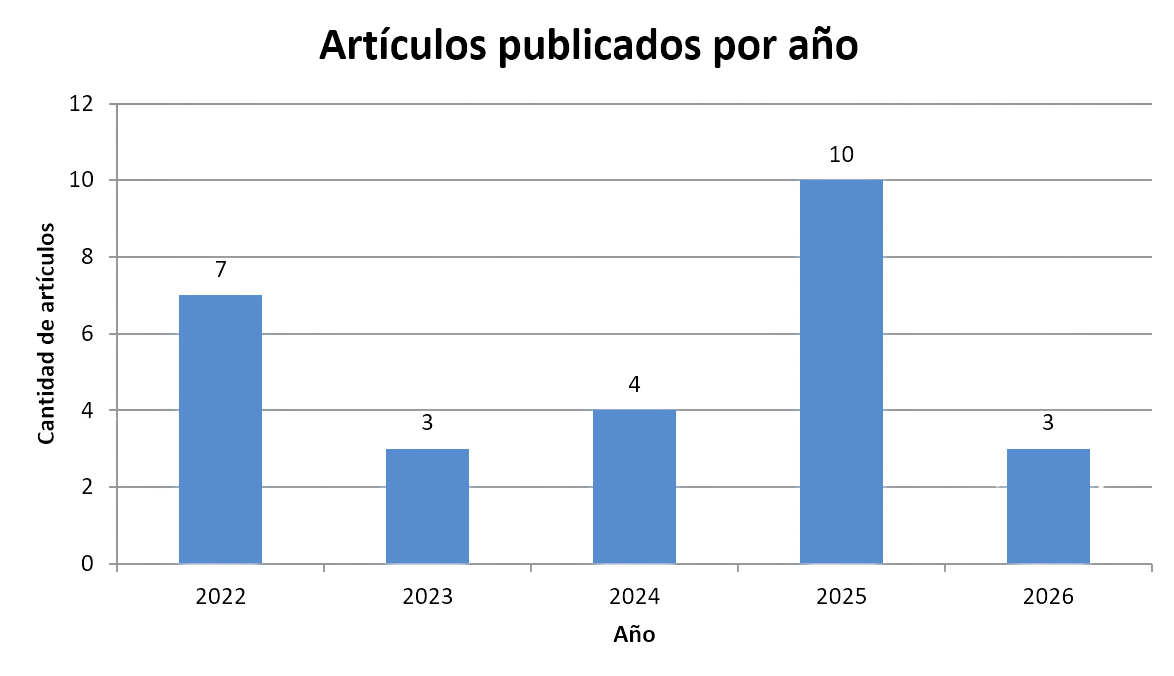
\includegraphics[width=8cm]{figures/fig3.png}
\end{center}
\caption{Artículos científicos por año}
\label{figura3}
\end{figure}


\begin{figure}[H]
\begin{center}
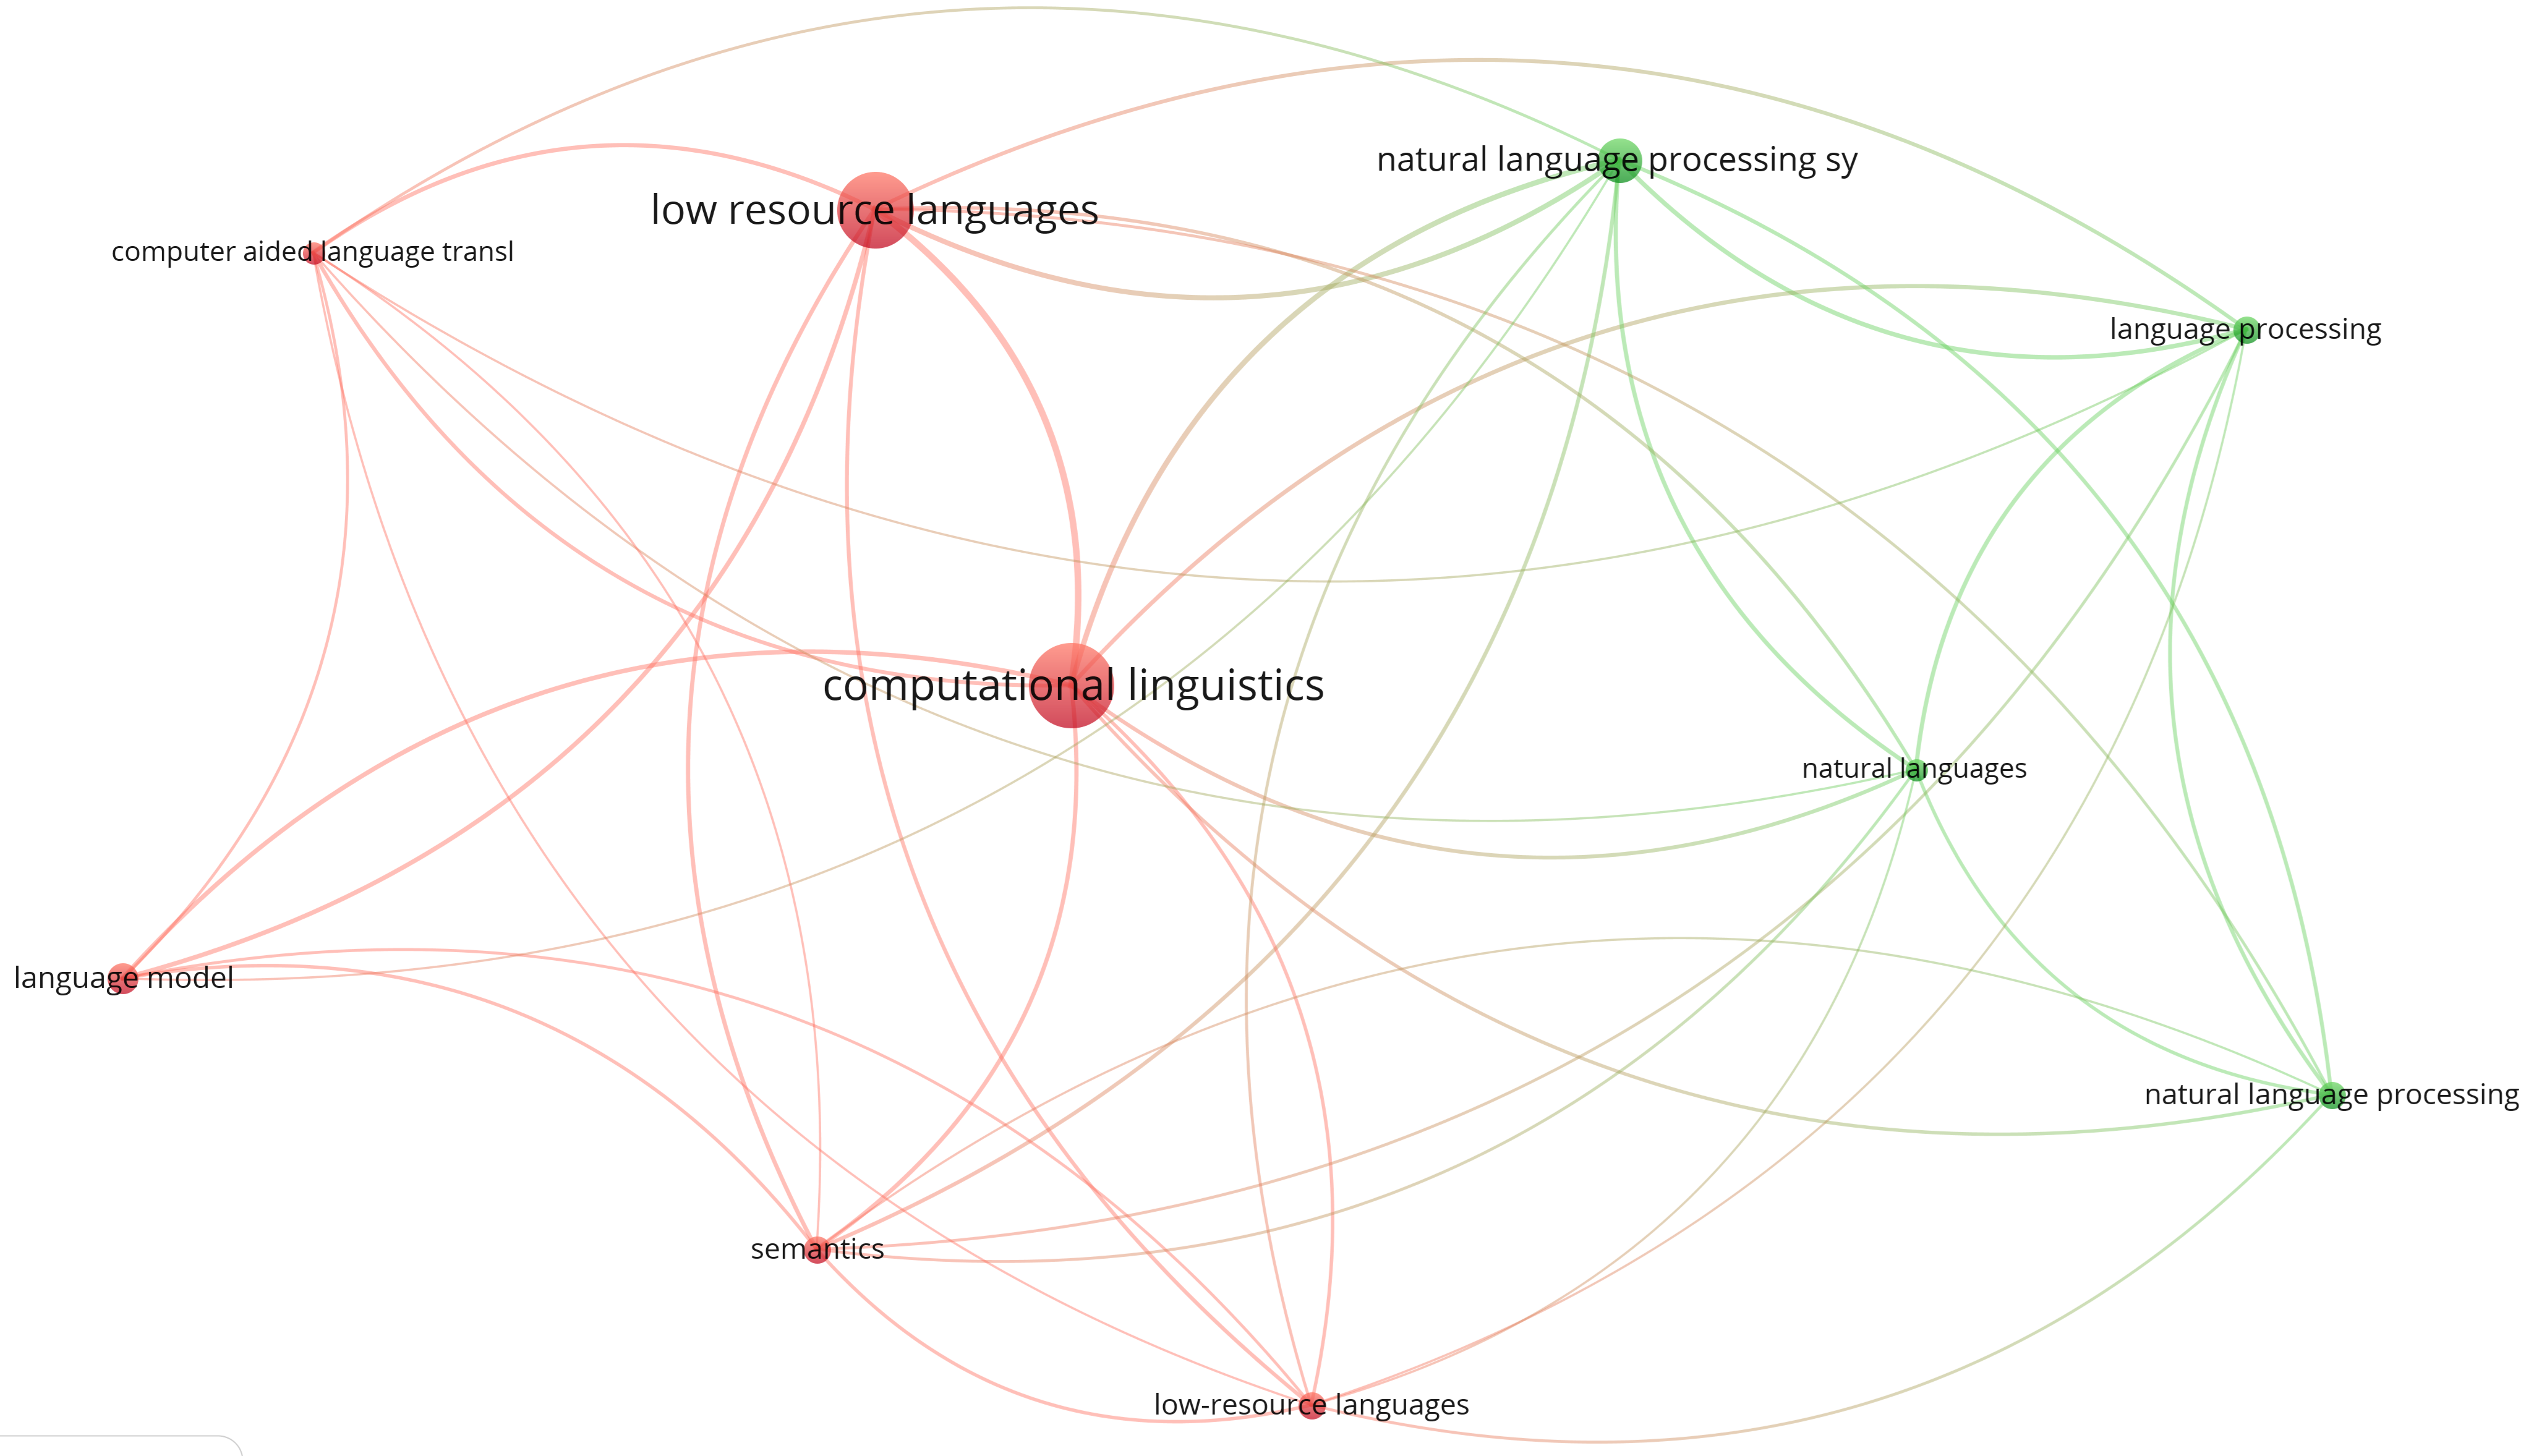
\includegraphics[width=8cm]{figures/fig4.png}
\end{center}
\caption{Red de coocurrencia de palabras clave}
\label{figura4}
\end{figure}

La figura 3 presenta la red de coocurrencia, la cual evidencia cómo se relacionan las palabras clave dentro de los artículos analizados. Se estableció un umbral de un mínimo de 5 ocurrencias por término, de las cuales solo 10 de 256 cumplieron este criterio. Asimismo, los conceptos con mayor centralidad son \textit{computational linguistics} con 19 ocurrencias, y \textit{low resource languages} con 17 ocurrencias; la proximidad entre ambos nodos y la mayor densidad de enlace, reflejan la alta frecuencia de aparición conjunta de ambas palabras clave. Por otro lado, es posible identificar por los colores rojo y verde la división entre dos grupos: el primero (rojo), agrupa las palabras orientadas a modelos, semántica y lenguajes de bajos recursos; mientras que el segundo (verde), destaca por su relación con el Procesamiento de Lenguaje Natural (NLP).

\begin{figure}[H]
\begin{center}
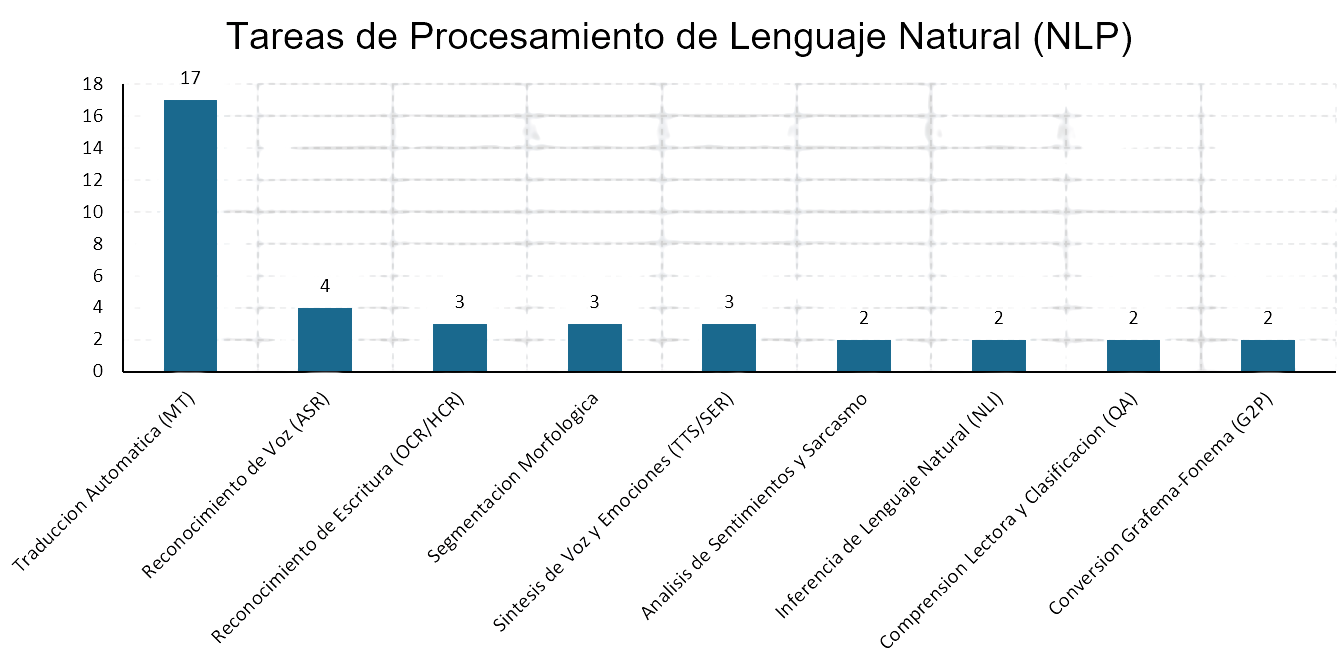
\includegraphics[width=8cm]{figures/fig5.png}
\end{center}
\caption{Tareas de Procesamiento de Lenguaje Natural (NLP)}
\label{figura5}
\end{figure}

\begin{figure}[H]
\begin{center}
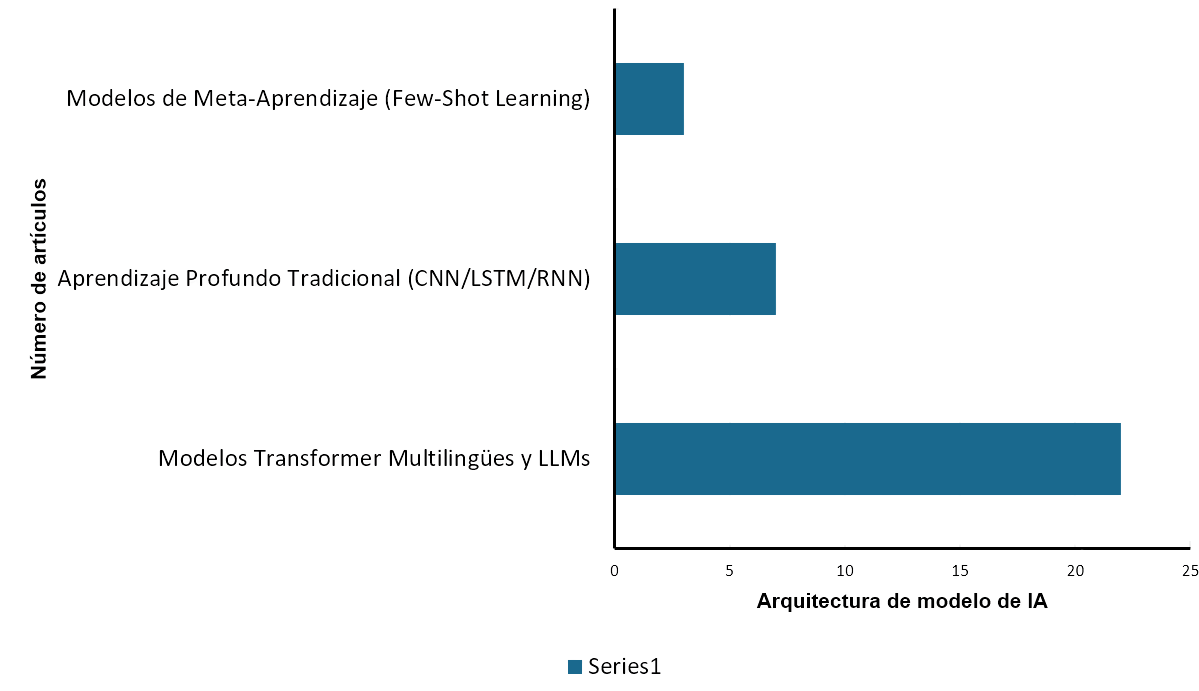
\includegraphics[width=8cm]{figures/fig6.png}
\end{center}
\caption{Arquitecturas y Modelos de Inteligencia Artificial}
\label{figura6}
\end{figure}

\begin{figure}[H]
\begin{center}
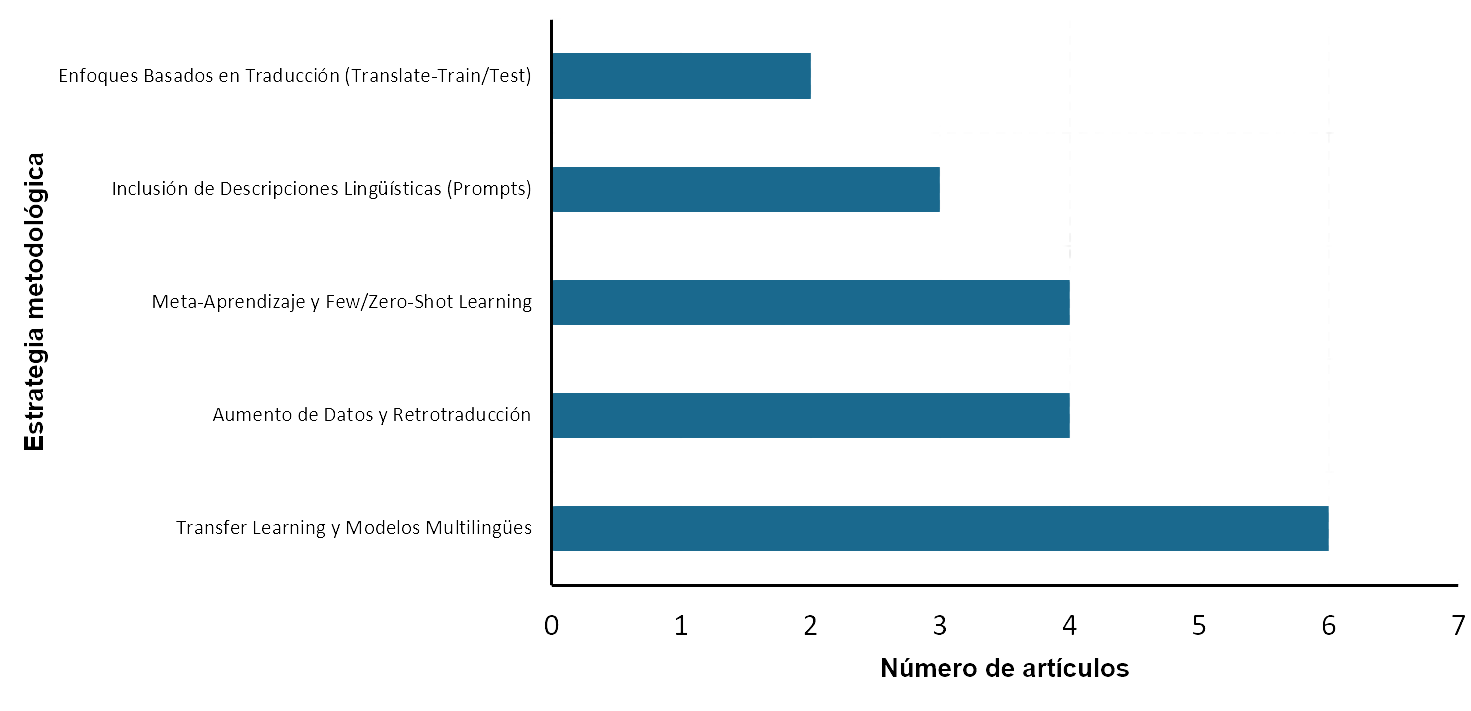
\includegraphics[width=8cm]{figures/fig7.png}
\end{center}
\caption{Estrategias para Mitigar la Escasez de Datos}
\label{figura7}
\end{figure}


\subsection{Resultados de ingeniería}
[Por completar]

% Estos dos apartados suelen aparecer juntos en muchos trabajos. No se deben confundiCoocurrenciacr esta discusión o análisis con la obtención de conclusiones, algo que depende tanto de los resultados y de su análisis como del marco teórico y de los objetivos.

% El pseudocódigo de los algoritmos debe ser presentado según indica el ejemplo del algortimo

% \begin{algorithm}[H]
% \label{algo1}
% \SetAlgoLined
% \text{\textbf{Entrada:}} \text{Caso estudio}\\
% \text{\textbf{Salida:}} \text{Global solución}\\
% \KwResult{Escribir aquí el resultado }
%  initialización\;
%  \While{While condicion}{
%   instructions\;
%   \eIf{condición}{
%    instrucciones1\;
%    instrucciones2\;
%    }{
%    instrucciones3\;
%   }
%  }
%  \caption{Como escribir algoritmos}
% \end{algorithm}





%========================================================

\section{Conclusiones}
Esta revisión tuvo como objetivo sintetizar los enfoques metodológicos empleados, resultados educativos reportados e identificar los principales desafíos y oportunidades. Los hallazgos evidencian que la inteligencia artificial aplicada a lenguas de bajos recursos se encuentra en crecimiento, aunque todavía presenta una producción científica limitada y dispersa. No obstante, se identificó un incremento en las publicaciones del año 2024 al 2025. Asimismo, la mayor parte de las publicaciones corresponde a investigaciones experimentales y propuestas de modelos las cuales representan el 66.7\% del total de la muestra. 

En cuanto a aplicaciones educativas, los resultados muestran que aplicaciones basadas en NLP contribuyen positivamente a integrar la lengua materna en entornos de aprendizaje con resultados más satisfactorios que los de una enseñanza tradicional. Por otro lado, entre las estrategias más utilizadas para enfrentar la falta de corpus y mejorar el desempeño de los modelos, se identifica el uso de descripciones lingüísticas, diccionarios mediante \textit{in-context learning} y técnicas de meta-aprendizaje. A su vez, otro hallazgo relevante es la existencia de brechas significativas en cuanto al rendimiento de herramientas basadas en IA entre lenguas de alto recurso y lenguas de bajos recursos, se reportaron distintas limitantes en tareas de comprensión semántica, traducción automática, seguimiento de instrucciones, seguridad y confiabilidad de los modelos.
En relación con las estrategias metodológicas, se evidenció que los enfoques más destacables combinan técnicas algorítmicas con metodologías participativas, como el \textit{transfer learning}, modelos multilingües, aumento de datos, meta-aprendizaje, arquitecturas híbridas y la inyección de conocimiento lingüístico. Sin embargo, también se resalta la importancia de involucrar a la población de estudio en el diseño y evaluación de las herramientas a fin de evitar la distorsión del conocimiento, respetar la soberanía sobre los datos y asegurar que las soluciones respondan a sus necesidades.
Finalmente, esta revisión sistemática de la literatura identifica desafíos que deben ser abordados en futuras investigaciones, entre ellas se encuentran la escasez de corpus digitalizados, dependencia excesiva de métricas como BLEU, TER o WER, la falta de inclusión de más de una variante dialectal, ausencia de ortografías estandarizadas y la complejidad morfofonémica. Aunque la inteligencia artificial representa una vía prometedora para mejorar la accesibilidad educativa en lenguas de bajos recursos, su implementación requiere enfoques más participativos que involucren a la población de estudio, prioricen sus necesidades y también tener en cuenta la variedad dialectal. La participación de hablantes nativos podría contribuir a crear mejores datos de entrenamiento y evitar errores culturales o de significado.



% Las conclusiones deben obtenerse, por tanto, a partir de algo más que de los simples datos registrados. De hecho, unos datos o resultados pueden tener un sentido u otro y, por tanto, pueden llevar a unas conclusiones y otras, dependiendo del marco conceptual que justifica la investigación, de la metodología seguida, de los objetivos propuestos, etc.
%========================================================

\section*{Agradecimientos}

[Por completar]
% Este apartado es opcional que dependerá su utilización en caso de exister algun organismo financiador, colaborador, etc., que permitió llevar a cabo la investigación.
%========================================================



\bibliography{referencias.bib}
\bibliographystyle{IEEEtran}
\end{multicols}
\end{document}